\section{Coherent Synchrotron Radiation}
Synchrotron radiation (SR) is produced in synchrotron radiation facilites (like electron storage rings) by accelerating relativistic electrons. Emission of  SR occurs, when bending/deflecting the electrons in dipole magnets or undulators\footnote{Undulators are used to make the electrons oscillate by generating a periodic magnetic field}. 

\autoref{fig:storageRing} shows a general scheme of an electron storage ring. Electrons, or rather electron bunches, are generated with an electron gun and are accelerated to almost speed of light by a linear accelerator (LINAC). The bunches are injected into the storage ring, after reaching their nominal energy in a booster. In the ring, the path of the electron bunches is altered by bending magnets, leading them on a circular trajectory. Due to emission of SR at each bending, the electrons lose energy, which has to be compensated. This is done in an accelerating radiofrequency (RF) cavity. Not shown in the scheme are the beamlines, which lead the SR radiation, or rather chosen wavelength regions of it, through an optical system to the respective user experiments.\cite{roussel2014} \cite{rota2018}

 \begin{figure}[H]
 	\centering
 	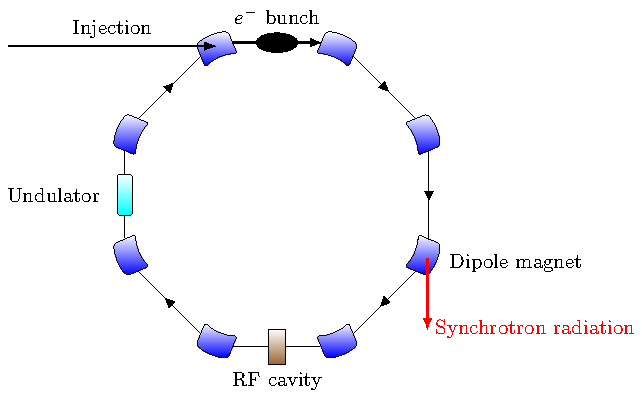
\includegraphics[width=0.7\textwidth]{chap/02-theory/img/synchrotron}
 	\caption{Basic scheme of an electron storage ring (redrawn from \cite{roussel2014})}
 	\label{fig:storageRing}
 \end{figure}
The range of SR reaches from hard X-rays down to the infrared region of the electromagnetic spectrum (see \autoref{fig:spectrum}). In contrast to other sources, it has properties like:
\begin{itemize}[noitemsep]
	\item high intensity 
	\item high collimation
	\item polarisation
	\item well-defined timing of pulses
\end{itemize}

Due to this properties, synchrotrons are used for microscopy, spectroscopy, and time-resolved experiments in such fields like condensed matter physics, biology, material science and many more. 
\begin{figure}[H]
	\centering
	\includegraphics[width = 0.8\textwidth, height = 0.5\textwidth]{chap/02-theory/img/spectrum.tikz}
	\caption{Electromagnetic spectrum}
	\label{fig:spectrum}
\end{figure}
As demands in these fields are ever-increasing, electron accelerators need to provide higher brilliance (or brightness). This is achieved by increased photon flux and reduction of the transverse emittance. For longidutinal coherence, the electron bunches are shortened, which results in emission of coherent synchrotron radiation (CSR) at frequencies up to the THz range. However, this introduces complex dynamics, as the electrons interact with their own radiation. This manifests into the so called microbunching instability: the formation of microstructures (in the sub-millimeter to centimeter range) in the longitudinal density profile of the electron bunches. Being on the one side a limitation to the stable operation of the overall system at high current density/short bunch length mode. On the other side, these instabilities can be potential sources of brilliant THz radiation. A thorough understanding of these dynamics is necessary to control the emission in this spectral domain which enables usage in experiments. \cite{rota2018} \cite{brosi}

\begin{figure}[H]
	\centering
	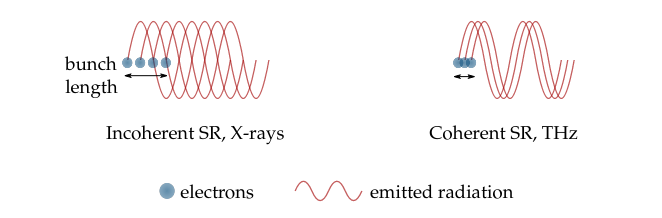
\includegraphics[width = 0.7\textwidth]{chap/02-theory/img/csr2.png}
	\caption{CSR \cite{rota2018}}
	\label{fig:csr}
\end{figure}

\begin{figure}[H]
	\centering
	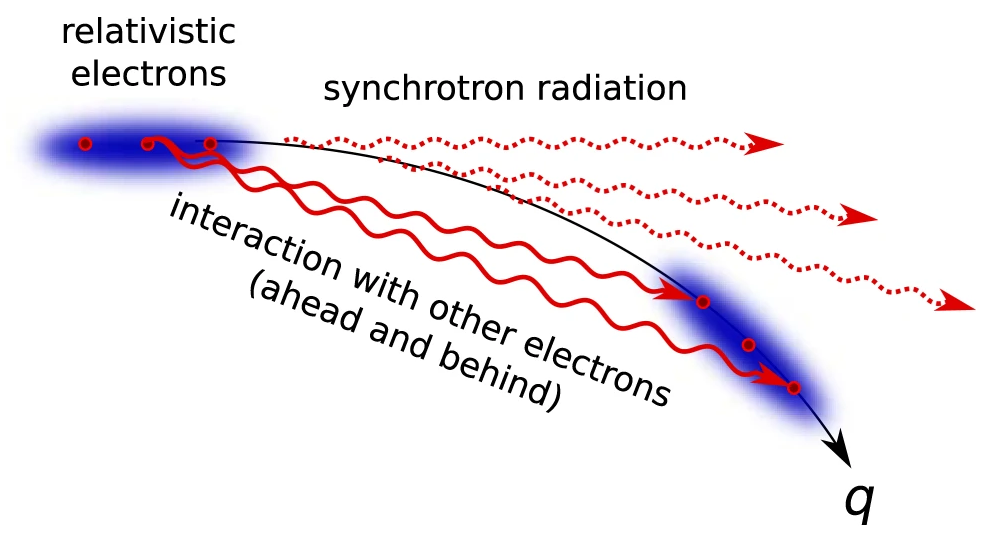
\includegraphics[width = 0.5\textwidth]{chap/02-theory/img/microbunching}
	\caption{Electrons interact with their own radiation \cite{Bielawski2019}}
	\label{fig:microBunch}
\end{figure}









\paragraph{KARA}
\begin{itemize}
	\item Located at the Karlsruhe Institute of Technology (KIT)
	\item Up to 184 electron packages (bunches) can be filled with a distance of \SI{2}{\nano \second} (\SI{500}{\mega \hertz}) between two adjacent bunches 
	\item Operated by the Institute of Beam Physics and Technology (IBPT)
	\item Microtron, Booster Synchrotron, and Storage Ring
\end{itemize}

\begin{table}[tbh!]
	\caption{KARA characteristics}
	\label{tab:kara}
	\begin{minipage}{\textwidth}
		\centering
		\begin{tabularx}{\textwidth}{XS}
			\toprule
			\textbf{Beam energy}     				& $ \SI{2.5}{\giga \electronvolt}$ \\
			\textbf{Circumference} 	 				& $\SI{110}{\meter}$	  \\
			\textbf{RF frequency }   				& $\SI{499.7}{\mega \hertz}$ 	\\
			\textbf{Harmonic number} 				& 184	\\
			\textbf{Number of RF stations} 			& 2 \\
			\textbf{Number of cavities per station} 	& 2	\\
			\textbf{Accelerating voltage} 					& $\SI{1.4}{\mega \electronvolt}$ \\
			\bottomrule		\end{tabularx}
	\end{minipage}
\end{table}



\begin{figure}[H]
	\centering
	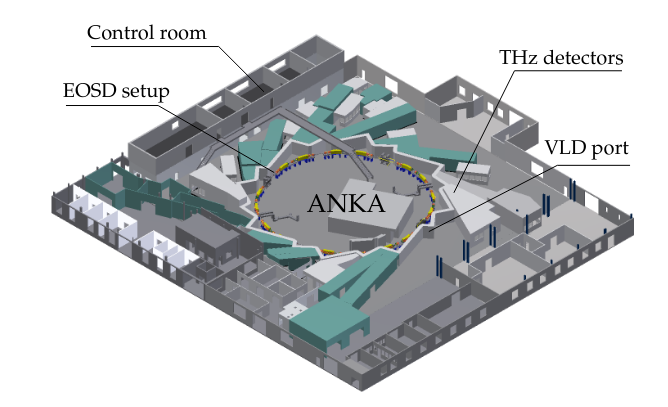
\includegraphics[width = 0.6\textwidth]{chap/02-theory/img/kara.png}
	\caption{Facility \cite{rota2018}}
	\label{fig:kara}
\end{figure}

\newpage 
\section{Photonic time-stretch analog-to-digital converter}










"' In recent and future synchrotron radiation facilities, relativistic electron bunches with increasingly high charge density are needed for producing brilliant light at various wavelengths, from X-rays to terahertz. In such conditions, interaction of electron bunches with their own emitted electromagnetic fields leads to instabilities and spontaneous formation of complex spatial structures. Understanding these instabilities is therefore key in most electron accelerators. However, investigations suffer from the lack of non-destructive recording tools for electron bunch shapes. In storage rings, most studies thus focus on the resulting emitted radiation. Here, we present measurements of the electric field in the immediate vicinity of the electron bunch in a storage ring, over many turns. For recording the ultrafast electric field, we designed a photonic time-stretch analog-to-digital converter with terasamples/second acquisition rate. We could thus observe the predicted link between spontaneous pattern formation and giant bursts of coherent synchrotron radiation in a storage ring. "'  \cite{Bielawski2019}

\begin{figure}[H]
	\centering
	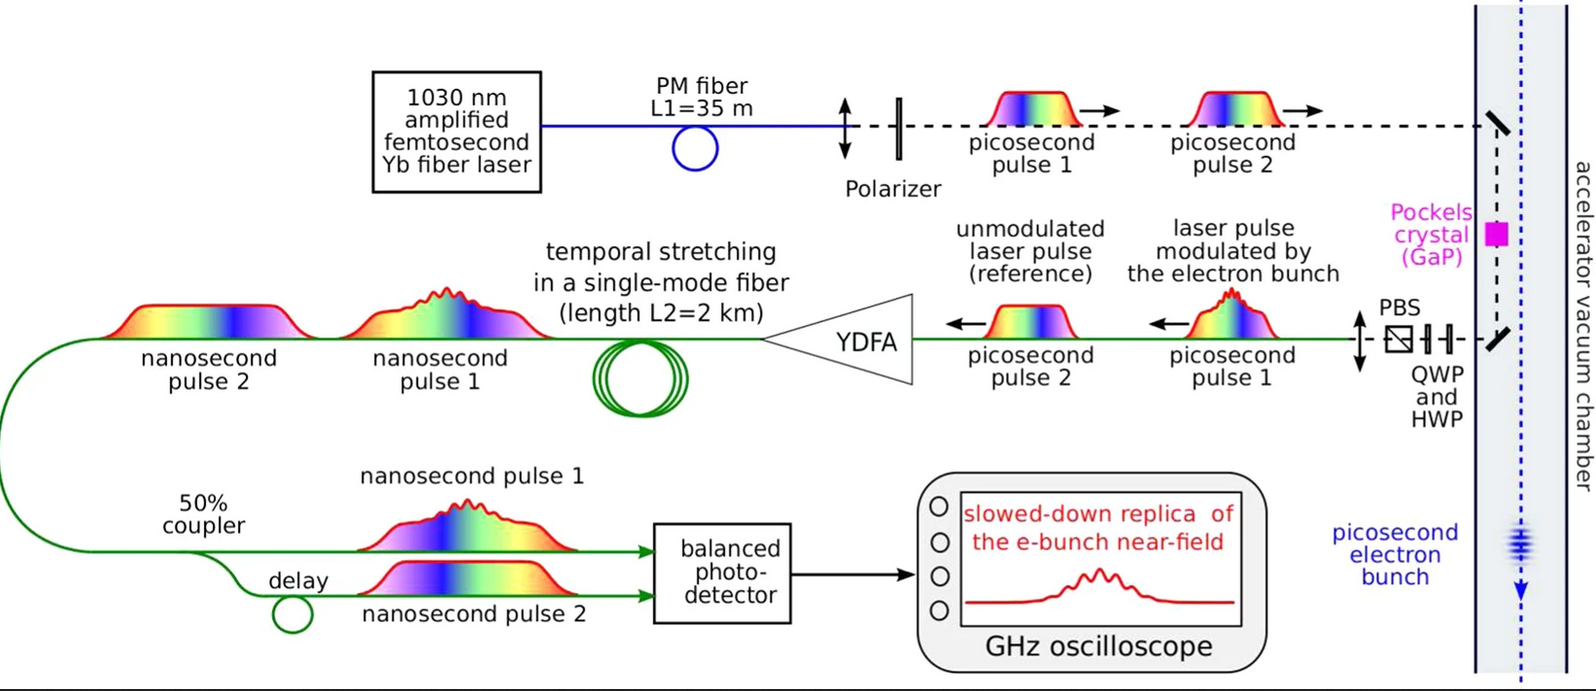
\includegraphics[width = 0.8\textwidth]{chap/02-theory/img/EO.png}
	\caption{Electro-Optical Time-Stretch Technique \cite{Bielawski2019}}
	\label{fig:eo}
\end{figure}


\newpage
\section{Characteristics of Analog-To-Digital-Converters}
Analog-to-digital converters (ADCs) are used to translate analog quantities into digital signals, which can be processed by information processing, computing, data transmission and control systems. This section covers the different characteristics of an ADC, which are needed to evaluate the performance of the convertes in the developed system. 
\subsection{Sampling Theory}

\paragraph{Nyquist-Criteria}
An ADC samples an analog signal with a frequency $f_s$. This frequency has to be chosen in such way, that the original signal can be fully reconstructed. The Nyquist criteria states, that in order to accurately represent a bandlimited, continous signal
\begin{equation}
y (t) \, \fourier  Y(f) \quad \text{with} \quad Y(f) = 0, \, |f| \geq \frac{B}{2}
\end{equation}
it has to be sampled with a frequency $f_s$ respecting
\begin{equation}
f_s \geq B \quad \text{or} \quad f_s \geq 2 f_a
\end{equation}
with $f_a$ being the highest frequency contained in the signal. \cite{walt} \cite{puente2015} \\
In other words, $f_a$ must be inside of the \textit{Nyquist bandwidth}, which is the spectrum from DC to $f_s/2$. Violation of this rule leads to \textit{aliasing}
\paragraph{Sample-And-Hold-Amplifier}
ADCs need a certain amount of time to sample the input signal. If the value of the signal changes by more than one Least-Significant-Bit (LSB) during this period, this can result in large errors in the output signal. Therefore, so called Sample-And-Hold-Amplifiers (SHA) are used in front of ADCs to hold the  input value for the needed amount of time. The ADC sampling time needs to be timed in such way, that the analog-to-digital conversion falls into the hold period of the SHA and doesn't exceed into the sample period, for example like shown schmeatically in the diagram below. Thus, the upper frequency limitation is not determined by the ADC itself, but rather by the aperture jitter,bandwidth, distortion, etc. of the SHA. \cite{walt}



\begin{figure} [H]
\centering
\tikzexternaldisable
\begin{tikztimingtable}
[%
    timing/dslope=0.1,
    timing/name/.style={font=\sffamily\normalsize},
    timing/d/text/.style={font=\sffamily\normalsize},
    grayz/.style={timing/z/.append style={gray}},
    timing/n/.style={rectangle},
    timing/metachar={{K}[2]{#1l !{++(0,+.5\yunit)} N[rectangle,scale=.6]{\shortstack{#2}} !{++(0,-.5\yunit)} #1l}},
    timing/metachar={{J}[2]{#1h !{++(0,-.5\yunit)} N[rectangle,scale=.6]{\shortstack{#2}} !{++(0,+.5\yunit)} #1h}},
  ]
 SHA & 1H 8K{HOLD} 8J{SAMPLE} 8K{HOLD} 3H\\
 Sampling & 5S A 16S A                    \\
\end{tikztimingtable}
\tikzexternalenable
\end{figure}

In addition to the SHA, there is also the Track-And-Hold-Amplifier (THA). Instead of a sample period, the THA has a track period, where the output of the amplifier tracks the input signal (see also \autoref{fig:tha}). When switching to hold mode, the signal at this instant is held. This is opposed to the SHA, where the output during sample mode is actually not defined and is set to the value of the input signal, only when switching into hold mode. 

\begin{figure}[H]
	\centering
	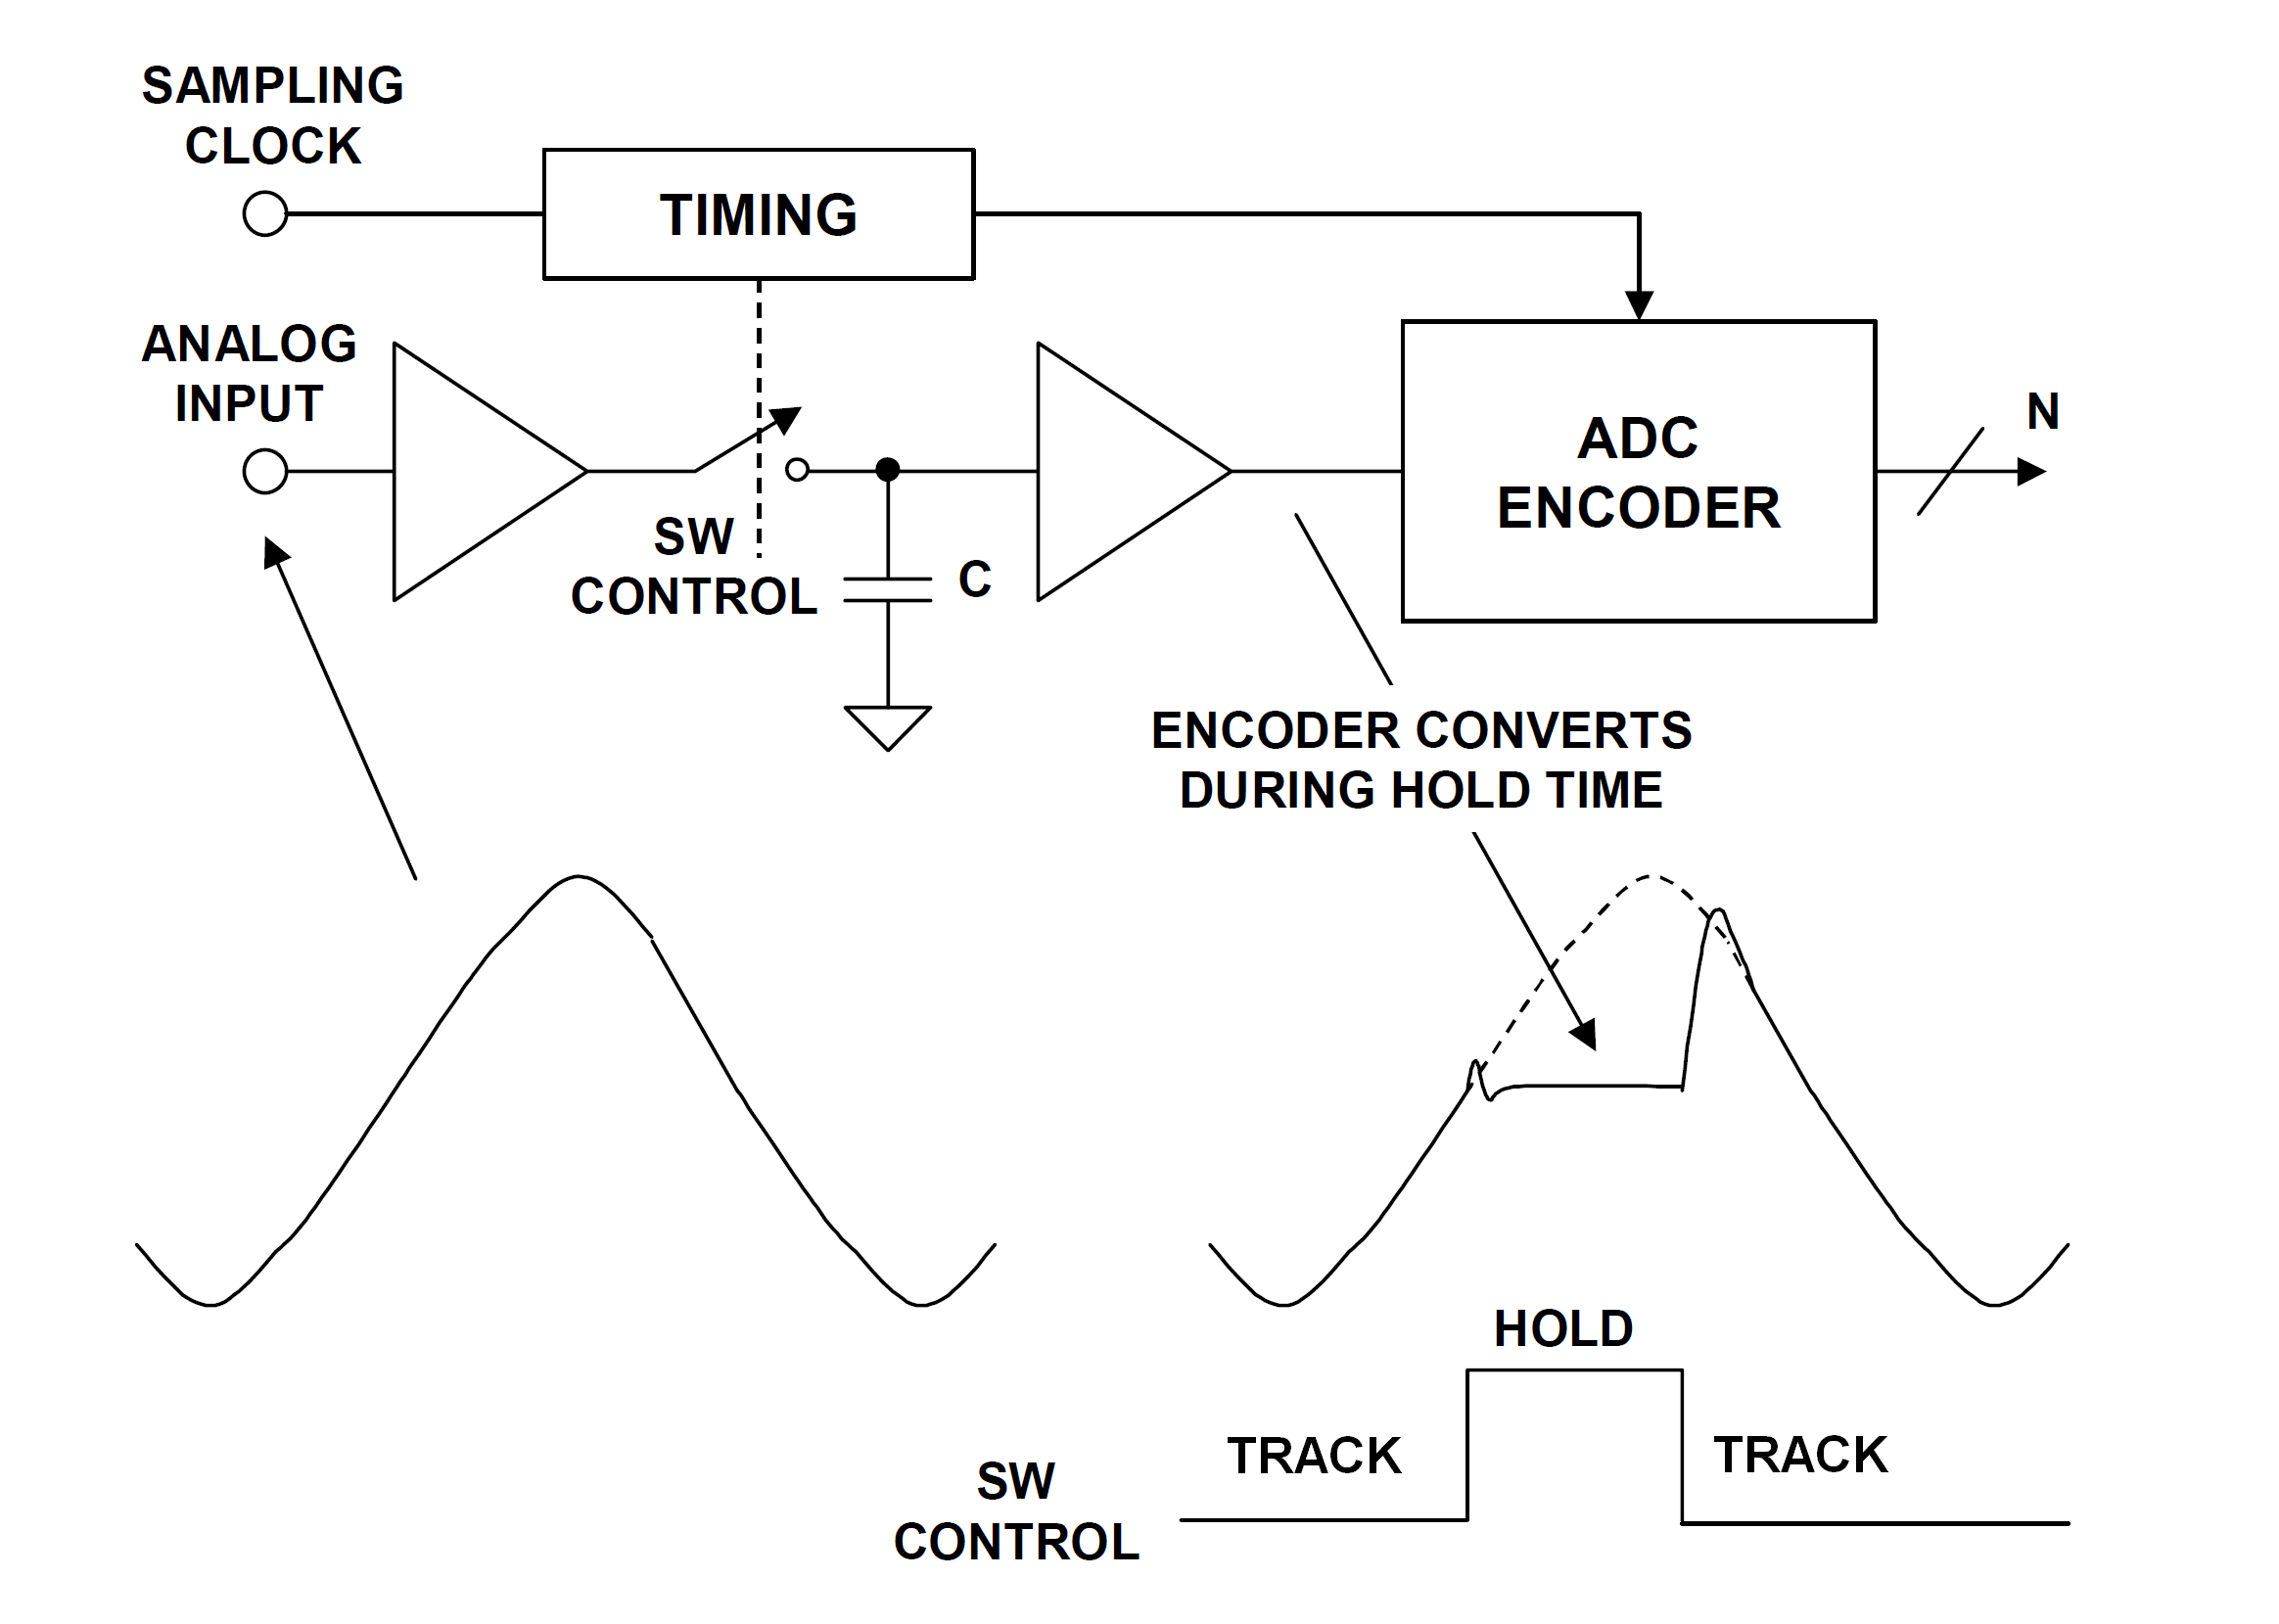
\includegraphics[width = 0.5\textwidth]{chap/02-theory/img/tha}
	\caption{Track-And-Hold-Amplifier schematic and principle \cite{walt}}
	\label{fig:tha}
\end{figure}
\subsection{AC errors}
In this section, the most important AC errors are briefly described.

\paragraph{Quantization Noise}
An ideal N-bit converter has errors occuring during sampling and quantization. For an equidistant quantization the \textbf{quantization error} is:
\begin{equation}
	\left| e_q(t) \right| = \left| x_q(t) - x(t) \right| \leq \frac{q}{2}
\end{equation}
with $x_q(t)$ being the quantized/discrete signal, $x(t)$ the input signal and $q$ the widht of the quantisation stage. \cite{puente2015}
In time domain, can be approximated with a sawtooth signal:
\begin{equation}
	e(t) = st, \quad -\frac{q}{2s} < t < \frac{q}{2s} 
\end{equation}
\begin{figure}[H]
	\centering
	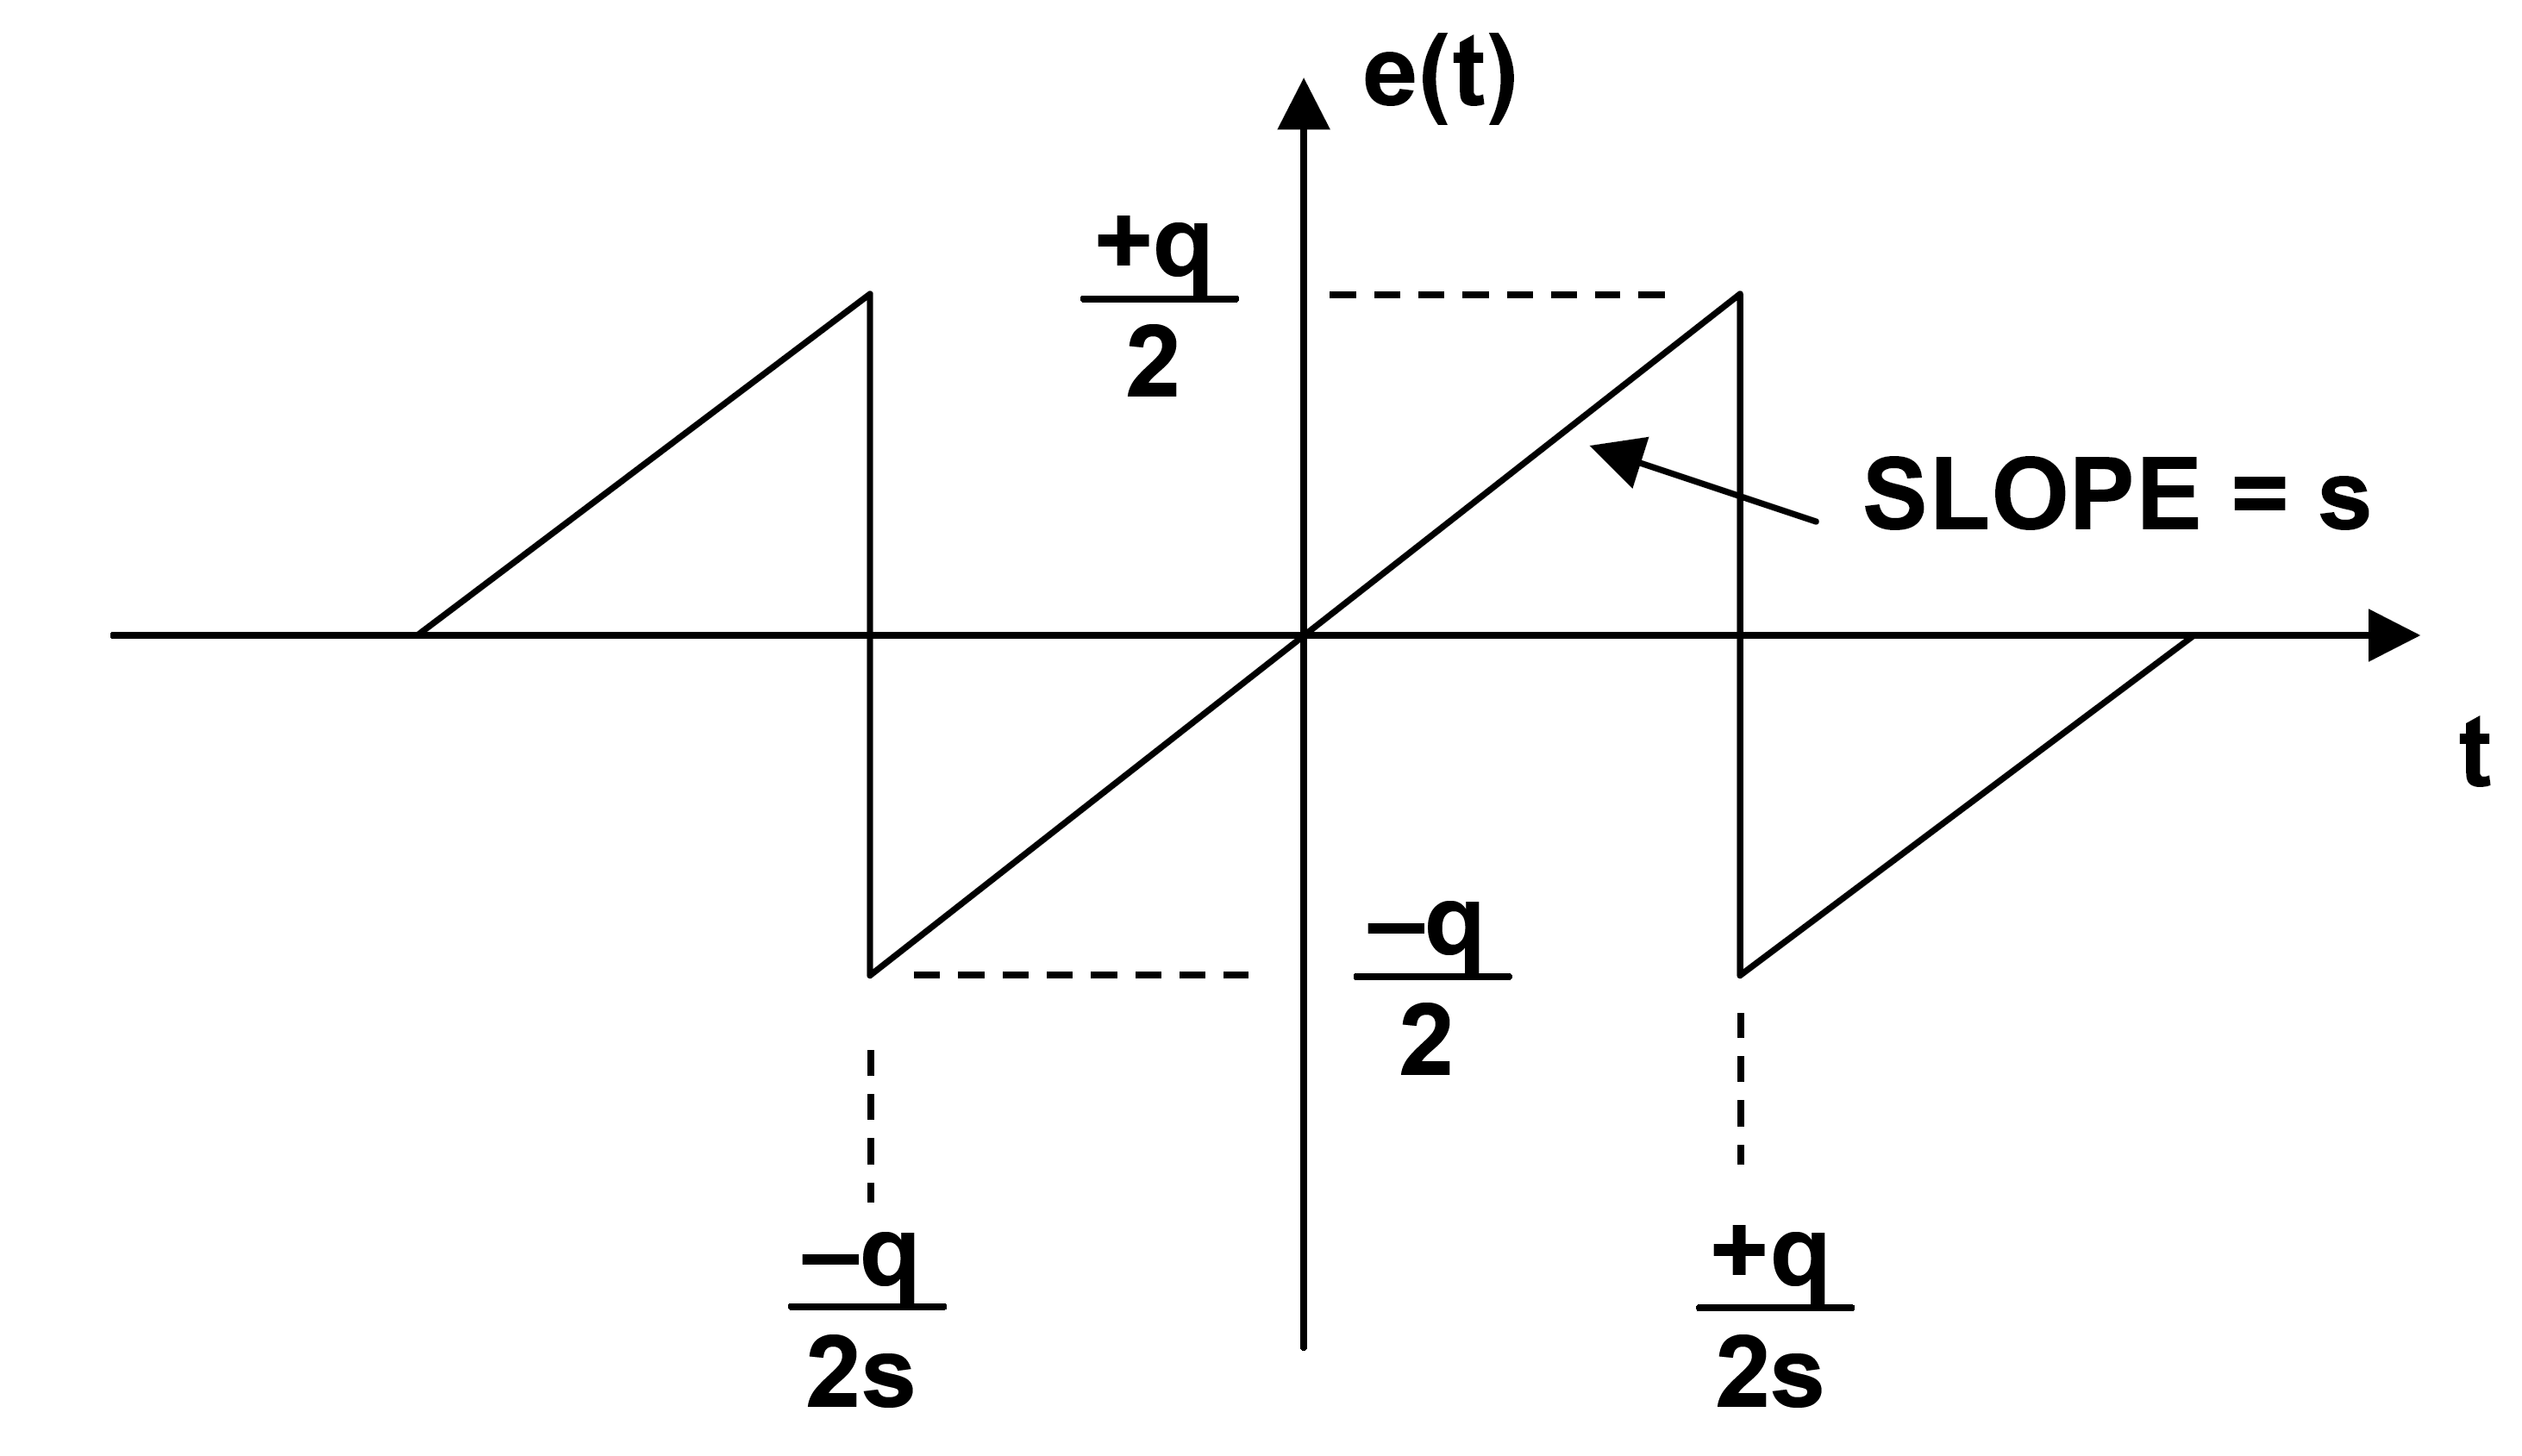
\includegraphics[width = 0.5\textwidth]{chap/02-theory/img/quantization_error}
	\caption{Quantization noise as function of time\cite{walt}}
	\label{fig:eq}
\end{figure}

The power of the quantization noise can be calculated as the mean-square of $e(t)$:
\begin{equation}
	P_{QN} = e_{\text{rms}}^{2} = \overline{e^{2}(t)} = \frac{s}{q}\int_{-q/2s}^{+q/2s} (st)^{2} dt = \frac{q^2}{12}
\end{equation}
The rms quantization error is then:
\begin{equation}
	e_{rms} = \frac{q}{\sqrt{12}}
\end{equation}

Assuming a full-scale input sinewave, the theoretical Signal-To-Noise-Ratio (SNR) of the ideal converter can be calculated as follows:
\begin{equation}
	\text{Sine wave:} \quad u(t) = u_s \sin(2\pi f t) = \frac{2^{N}q}{2}\sin(2\pi f t)
\end{equation}
\begin{equation}
	u_{\text{eff}} = \frac{u_s}{\sqrt{2}} = \frac{2^{N-1}q}{2}\sin(2\pi f t)
\end{equation}
\begin{equation}
	\text{SNR} = \frac{P_{\text{signal}}}{P_{\text{noise}}} = \frac{u_{\text{eff}}^{2}}{e_{\text{rms}}^{2}}
\end{equation}

\begin{itemize}
\item Equivalent Input Referred Noise
\item Noise-Free Code Resolution
\end{itemize}
\paragraph{Integral and Differential Nonlinearity Distortion} 

\paragraph{Dynamic Performance}

\begin{itemize}
\item Harmonic Distortion, Worst Harmonic, Total Harmonic Distortion (THD), Total Harmonic Distortion + Noise (THD + N)
\item Signal-to-Noise-and-Distortion Ratio (SINAD, or S/N + D), Signal-to-Noise ratio (SNR), Effective Number of Bits (ENOB)
\item Analog Bandwidth (Full-Power, Small-Signal)
\item Spurious Free Dynamic Range (SFDR)
\item Two-Tone Intermodulation Distortion, Multi-Tone Intermodulation Distortion
\item Noise Power Ratio (NPR)
\item Adjacent Leakage Ratio (ACLR)
\item Noise Figure
\item Setting Time, Overvoltage Recovery Time
\end{itemize}

\cite{walt}
\subsection{Interleaving}

\begin{itemize}
\item Net sample rate
\item Interleaving Spurs
\end{itemize}

\cite{mangrob}




\newpage
\section{RF/Microwave Design Basics}